%auto-ignore
\documentclass[tikz]{standalone}

\begin{document}
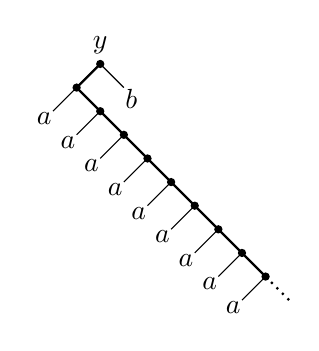
\begin{tikzpicture}[scale=0.3]

\draw (1,-1) node [below right=-0.3em] {$b$}
-- (0,0) node [above] {$y$}
-- (-1,-1) -- (7,-9);

\fill (0,0) circle (5pt);

\foreach \x in {-1,0,1,2,3,4,5,6,7} {
	\draw (\x,-2-\x) to +(-1,-1) node [below left=-0.3em] {$a$};
	\fill (\x,-2-\x) circle (5pt);
}

\draw [dotted,thick] (7,-9) to +(1,-1);
\draw [thick] (0,0) to ++(-1,-1) to ++(8,-8);

\end{tikzpicture}
\end{document}